\باب{سوالات}
%========================
\ابتدا{سوال}\شناخت{سوال_فوریئر_چکور_الف}
شکل \حوالہ{شکل_سوال_فوریئر_چکور_الف}-الف کے  عددی سر حاصل کرتے ہوئے اس کی تکونیاتی فوریئر تسلسل لکھیں۔
\begin{figure}
\centering
\begin{subfigure}{0.5\textwidth}
\centering
\begin{tikzpicture}
\begin{axis}[small,xtick={0,0.2,1,1.2},xticklabels={$0$,$0.2$,$1$,$1.2$},ytick={0,1},yticklabels={$0$,$1$},xlabel={$t$},ylabel={$v(t)$},ylabel style={rotate=-90},ylabel style={at={(axis description cs:0,1.05)}}]
\addplot[] plot coordinates {(-0.1,0) (0,0) (0,1) (0.2,1) (0.2,0) (1,0) (1,1) (1.2,1) (1.2,0) (1.5,0)};
\end{axis}
\end{tikzpicture}
\caption*{(الف)}
\end{subfigure}%
\begin{subfigure}{0.5\textwidth}
\centering
\begin{tikzpicture}
\begin{axis}[small,xtick={0,3,6,9,12},xticklabels={$0$,$3$,$6$,$9$,$12$},ytick={-1,0,1},yticklabels={$-1$,$0$,$1$},xlabel={$t$},ylabel={$i(t)$},ylabel style={rotate=-90},ylabel style={at={(axis description cs:0,1.05)}}]
\addplot[] plot coordinates {(-0.5,-1) (0,-1)(0,1)(3,1)(3,-1)(6,-1) (6,1) (9,1) (9,-1) (12,-1) (12,1) (12.4,1)};
\end{axis}
\end{tikzpicture}
\caption*{(ب)}
\end{subfigure}%
\caption{سوال \حوالہ{سوال_فوریئر_چکور_الف} کی موج۔}
\label{شکل_سوال_فوریئر_چکور_الف}
\end{figure}

جوابات:\عددی{a_0=0.2}، \عددی{a_n=\tfrac{1}{n\pi}\sin \tfrac{2\pi n}{5}}، \عددی{b_n=\tfrac{1}{n\pi}(1-\cos \tfrac{2\pi n}{5})}، \\
\begin{multline*}
v(t)=0.2+0.3027\cos (2\pi t) +0.2199\sin (2\pi t)+0.0935\cos(4\pi t)\\
+0.2879\sin(4\pi t)-0.0623\cos(6\pi t)+0.1919\sin(6\pi t)+\cdots
\end{multline*}
\انتہا{سوال}
%=========================
\ابتدا{سوال}\شناخت{سوال_فوریئر_چکور_ب}
شکل \حوالہ{شکل_سوال_فوریئر_چکور_الف}-ب کے تکونی فوریئر تسلسل کے عددی سر حاصل کریں۔تسلسل کے شروع کے چند ارکان لکھیں۔

جوابات:\عددی{a_0=0}، \عددی{a_n=0}، \عددی{b_n=\tfrac{2}{n\pi}(1-(-1)^n)}،
\begin{align*}
i(t)=\tfrac{4}{\pi}[\sin(\tfrac{\pi}{2}t)+\tfrac{1}{3}\sin(\tfrac{3\pi}{2}t)+\tfrac{1}{5}\sin(\tfrac{5\pi}{2}t)+\cdots]
\end{align*}
\انتہا{سوال}
%==========================
\ابتدا{سوال}\شناخت{سوال_فوریئر_چکور_پ}
شکل \حوالہ{شکل_سوال_فوریئر_چکور_پ}-الف کے  عددی سر حاصل کرتے ہوئے اس کی تکونیاتی فوریئر تسلسل لکھیں۔
\begin{figure}
\centering
\begin{subfigure}{0.5\textwidth}
\centering
\begin{tikzpicture}
\begin{axis}[small,xtick={0,1,2,3,4,5},xticklabels={$0$,$1$,$2$,$3$,$4$,$5$},ytick={0,1,2},yticklabels={$0$,$1$,$2$},xlabel={$t$},ylabel={$v(t)$},ylabel style={rotate=-90},ylabel style={at={(axis description cs:0,1.05)}}]
\addplot[] plot coordinates {(-0.5,0)(0,0)(0,2)(1,2)(1,1)(2,1) (2,0) (3,0)(3,2)(4,2)(4,1)(5,1) (5,0) (5.5,0)};
\end{axis}
\end{tikzpicture}
\caption*{(الف)}
\end{subfigure}%
\begin{subfigure}{0.5\textwidth}
\centering
\begin{tikzpicture}
\begin{axis}[small,xtick={0,1,2,3,4,5,6,7},xticklabels={$0$,$1$,$2$,$3$,$4$,$5$,$6$,$7$},ytick={0,1,2},yticklabels={$0$,$1$,$2$},xlabel={$t$},ylabel={$i(t)$},ylabel style={rotate=-90},ylabel style={at={(axis description cs:0,1.05)}}]
\addplot[] plot coordinates {(-0.5,0)(0,0)(0,1)(1,1)(1,2)(2,2) (2,1) (3,1)(3,0)(4,0)(4,1)(5,1) (5,2) (6,2) (6,1) (7,1) (7,0) (7.5,0)};
\end{axis}
\end{tikzpicture}
\caption*{(ب)}
\end{subfigure}%
\caption{سوال \حوالہ{سوال_فوریئر_چکور_پ} کی موج۔}
\label{شکل_سوال_فوریئر_چکور_پ}
\end{figure}

جوابات:
\begin{align*}
a_0&=1\\
a_n&=0\\
b_n&=\tfrac{3}{\pi}, \tfrac{3}{2\pi}, 0, \tfrac{3}{4\pi}, \tfrac{3}{5\pi}, 0, \tfrac{3}{7\pi}, \cdots\\
i(t)&=1+\tfrac{3}{\pi}(\sin \tfrac{2\pi t}{3}+\tfrac{1}{2}\sin \tfrac{4\pi t}{3}+\tfrac{1}{4}\sin \tfrac{8\pi t}{3}+\cdots)
\end{align*}
\انتہا{سوال}
%=========================
\ابتدا{سوال}\شناخت{سوال_فوریئر_چکور_ت}
شکل \حوالہ{شکل_سوال_فوریئر_چکور_پ}-ب کے تکونی فوریئر تسلسل کے عددی سر حاصل کریں۔تسلسل کے شروع کے چند ارکان لکھیں۔

جوابات:
\begin{align*}
a_0&=1\\
a_n&=-\tfrac{2}{\pi},0,\tfrac{2}{3\pi},0,-\tfrac{2}{5\pi},0,\tfrac{2}{7\pi},\cdots\\
b_n&=\tfrac{2}{\pi},0,\tfrac{2}{3\pi},0,\tfrac{2}{5\pi},0,\tfrac{2}{7\pi},\cdots\\
i(t)&=1-\tfrac{2}{\pi}(\cos \tfrac{\pi t}{2}-\sin \tfrac{\pi t}{2}-\tfrac{1}{3}\cos \tfrac{3\pi t}{2}-\tfrac{1}{3}\sin \tfrac{\pi t}{2}+\cdots  )
\end{align*}
\انتہا{سوال}
%==========================
\ابتدا{سوال}\شناخت{سوال_فوریئر_چکور_ٹ}
شکل \حوالہ{شکل_سوال_فوریئر_چکور_ٹ}-الف کے  عددی سر حاصل کرتے ہوئے اس کی تکونیاتی فوریئر تسلسل لکھیں۔
\begin{figure}
\centering
\begin{subfigure}{0.5\textwidth}
\centering
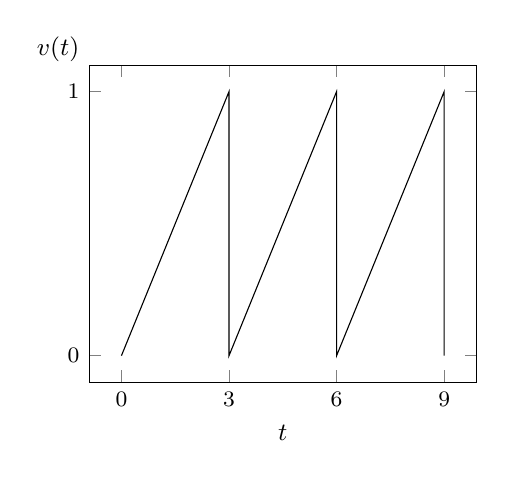
\begin{tikzpicture}
\begin{axis}[small,xtick={0,3,6,9},xticklabels={$0$,$3$,$6$,$9$},ytick={0,1},yticklabels={$0$,$1$},xlabel={$t$},ylabel={$v(t)$},ylabel style={rotate=-90},ylabel style={at={(axis description cs:0,1.05)}}]
\addplot[] plot coordinates {(0,0)(3,1)(3,0)(6,1)(6,0)(9,1)(9,0)};
\end{axis}
\end{tikzpicture}
\caption*{(الف)}
\end{subfigure}%
\begin{subfigure}{0.5\textwidth}
\centering
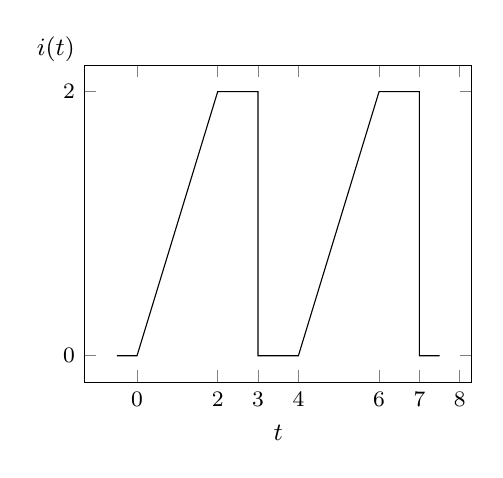
\begin{tikzpicture}
\begin{axis}[small,xtick={0,2,3,4,6,7,8},xticklabels={$0$,$2$,$3$,$4$,$6$,$7$,$8$},ytick={0,2},yticklabels={$0$,$2$},xlabel={$t$},ylabel={$i(t)$},ylabel style={rotate=-90},ylabel style={at={(axis description cs:0,1.05)}}]
\addplot[] plot coordinates {(-0.5,0)(0,0)(2,2)(3,2)(3,0)(4,0)(6,2)(7,2)(7,0)(7.5,0)};
\end{axis}
\end{tikzpicture}
\caption*{(ب)}
\end{subfigure}%
\caption{سوال \حوالہ{سوال_فوریئر_چکور_ٹ} کی موج۔}
\label{شکل_سوال_فوریئر_چکور_ٹ}
\end{figure}

جوابات:
\begin{align*}
a_0&=\tfrac{9}{4}\\
a_n&=0\\
b_n&=-\tfrac{9}{2n\pi}\\
v(t)&=\tfrac{9}{4}-\tfrac{9}{2\pi}\sum_{n=1}^{\infty} \tfrac{1}{n}\sin \tfrac{2n\pi t}{3}
\end{align*}
\انتہا{سوال}
%=========================
\ابتدا{سوال}\شناخت{سوال_فوریئر_چکور_ث}
شکل \حوالہ{شکل_سوال_فوریئر_چکور_ٹ}-ب کے تکونی فوریئر تسلسل کے عددی سر حاصل کریں۔

جوابات:
\begin{align*}
a_0&=1\\
a_n&=-\tfrac{2}{\pi}(1+\tfrac{2}{\pi}), \tfrac{2}{3\pi}(1-\tfrac{2}{3\pi}), -\tfrac{2}{5\pi}(1+\tfrac{2}{5\pi}), \tfrac{2}{7\pi}(1-\tfrac{2}{7\pi}),-\cdots\\
b_n&=0,\tfrac{1}{\pi},0, -\tfrac{1}{2\pi},0,\tfrac{1}{3\pi},0,-\cdots
\end{align*}
\انتہا{سوال}
%==========================
